\documentclass[15pt,ngerman]{scrreprt}

\usepackage[utf8]{inputenc}
\usepackage[T1]{fontenc}
\usepackage{babel}

% für michas fotoalbum

\usepackage[landscape,left=1cm,right=1cm,bottom=2.5cm, top=1cm]{geometry}

\usepackage{subcaption}

% Beispieldefinition für \person{}

\newcommand{\person}[1]{\textsc{#1}}

\author{Uwe Ziegenhagen}
\title{Mein allererstes \LaTeX-Dokument}
%\date{1. Januar 2018}

\usepackage{blindtext}

\setlength{\parindent}{0pt}
\setlength{\parskip}{10pt}

\usepackage{microtype}
\usepackage{graphicx} % Bilder

\usepackage{paralist} %kompakte Aufzählungen

\usepackage{hyperref} % immer als letztes Paket

\hypersetup{
    bookmarks=true,                     % show bookmarks bar
    unicode=false,                      % non - Latin characters in Acrobat’s bookmarks
    pdftoolbar=true,                        % show Acrobat’s toolbar
    pdfmenubar=true,                        % show Acrobat’s menu
    pdffitwindow=false,                 % window fit to page when opened
    pdfstartview={FitH},                    % fits the width of the page to the window
    pdftitle={My title},                        % title
    pdfauthor={Author},                 % author
    pdfsubject={Subject},                   % subject of the document
    pdfcreator={Creator},                   % creator of the document
    pdfproducer={Producer},             % producer of the document
    pdfkeywords={keyword1, key2, key3},   % list of keywords
    pdfnewwindow=true,                  % links in new window
    colorlinks=true,                        % false: boxed links; true: colored links
    linkcolor=blue,                          % color of internal links
    filecolor=blue,                     % color of file links
    citecolor=blue,                     % color of file links
    urlcolor=blue                        % color of external links
}

\begin{document}
\maketitle

\tableofcontents

\listoffigures

\chapter{Das allererste Kapitel, los geht's}

\section{Einleitung des ersten Dokuments, was ich wo geschrieben hab}

\blindtext

Siehe Abbildung \ref{fig:ente} auf Seite \pageref{fig:ente}.

\section{Hauptteil}

\subsection{Einleitung zum Hauptteil}

Irgendein Text.

\subsubsection{Hauptteil}


\blindtext[2]

\blindtext[2]


\section{Fazit}

\begin{figure}[h]
	\begin{center}
		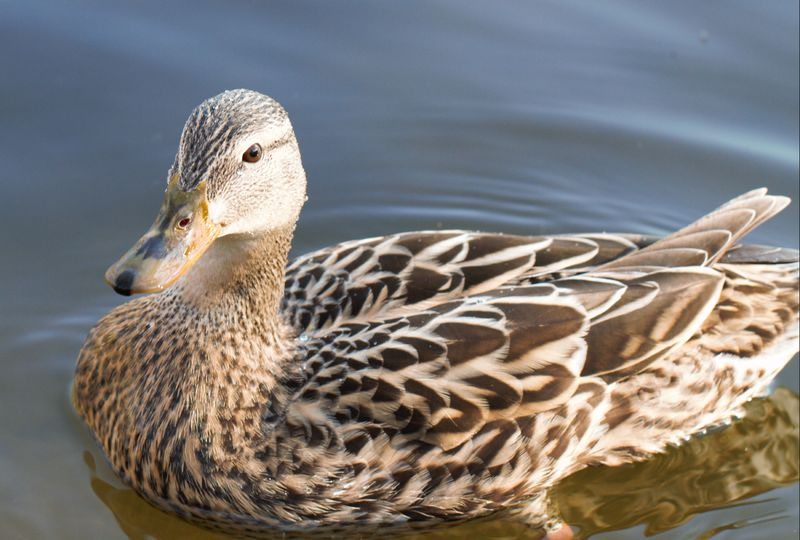
\includegraphics[width=0.75\textwidth]{./Bilder/image1}
	\caption{Meine erste Bildunterschrift}\label{fig:ente}
	\end{center}
\end{figure}


\begin{figure}[h]
	\begin{center}
		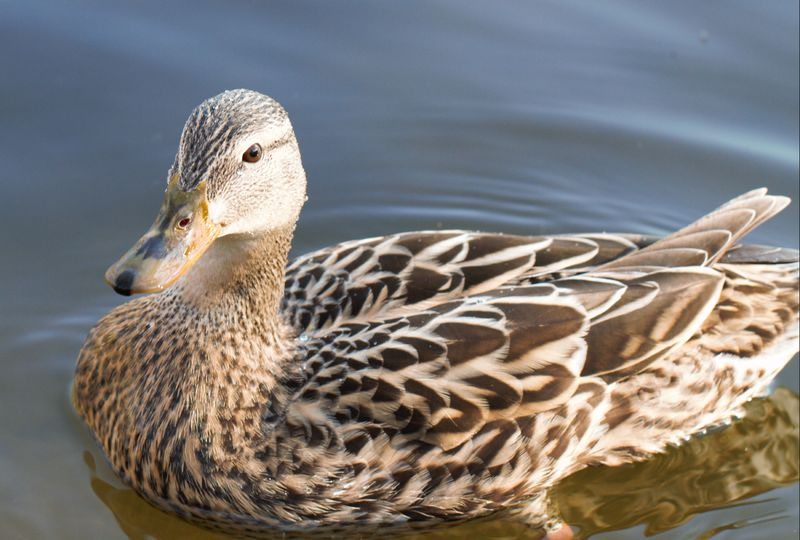
\includegraphics[width=0.75\textwidth]{./Bilder/image1}
	\caption{Meine erste Bildunterschrift}\label{fig:ente2}
	\end{center}
\end{figure}


\begin{figure}[h]
	\begin{center}
		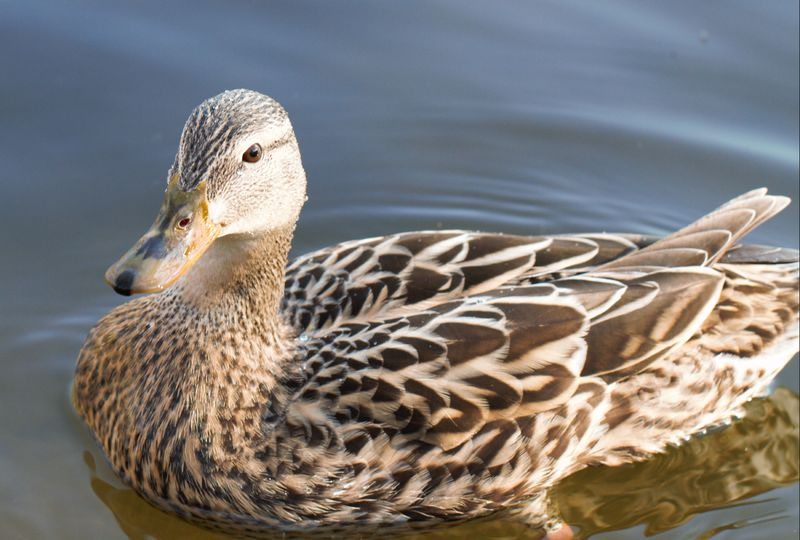
\includegraphics[width=0.75\textwidth]{./Bilder/image1}
	\caption{Meine erste Bildunterschrift}\label{fig:ente3}
	\end{center}
\end{figure}


\begin{figure}[h]
	\begin{center}
		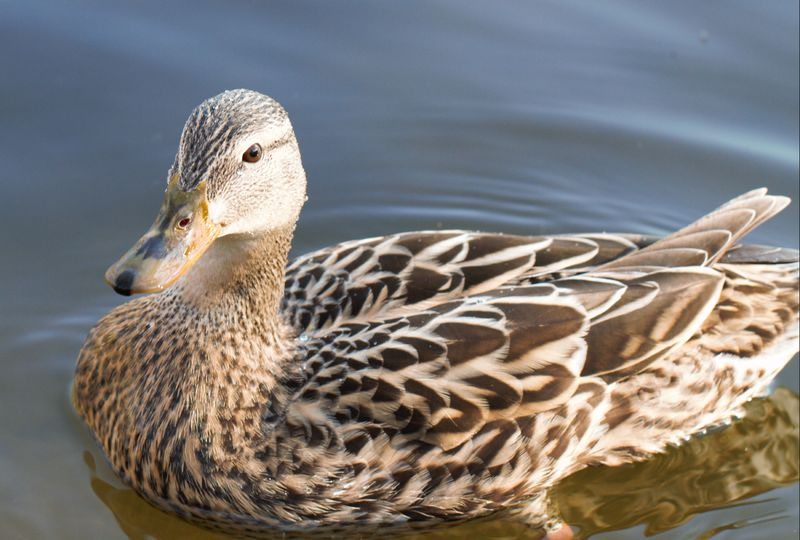
\includegraphics[width=0.75\textwidth]{./Bilder/image1}
	\caption{Meine erste Bildunterschrift}\label{fig:ente4}
	\end{center}
\end{figure}


\begin{figure}
\begin{subfigure}[c]{0.48\textwidth}

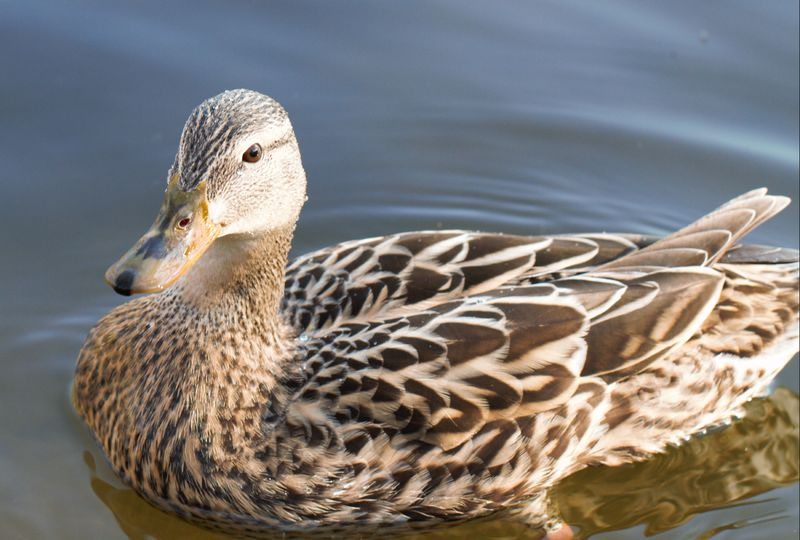
\includegraphics[width=\textwidth]{./Bilder/image1}
\subcaption{Subfigure Bild Nr. 1}

\end{subfigure}
\begin{subfigure}[c]{0.48\textwidth}
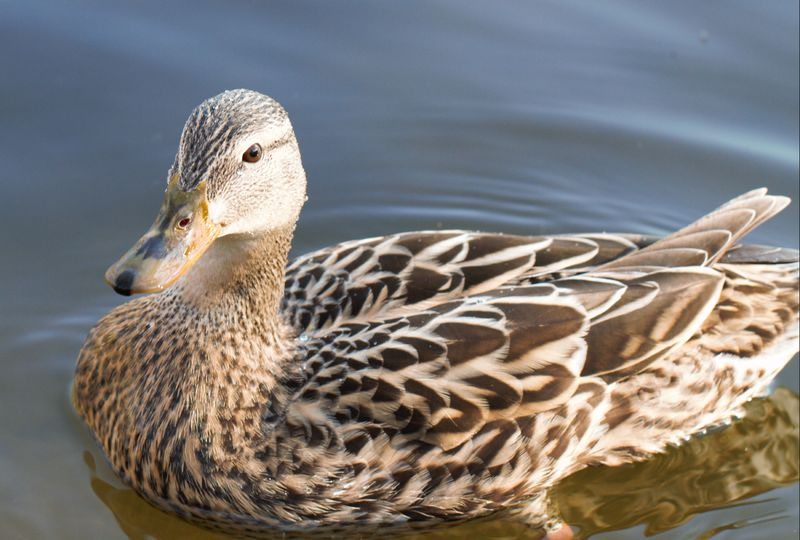
\includegraphics[width=\textwidth]{./Bilder/image1}
\subcaption{Subfigure Bild Nr. 2}
\end{subfigure}
\caption{Zwei Bilder mit Subfigure nebeneinander}
\end{figure}


\end{document}
